\documentclass{beamer}
\usepackage[utf8]{inputenc}
\usetheme{Madrid}
\usecolortheme{beaver}
\usepackage[style=british]{csquotes}


\usepackage{amsmath}
\usepackage{amsthm}
\usepackage{bm}

\newtheorem{prop}{Proposition}



\def\signed #1{{\leavevmode\unskip\nobreak\hfil\penalty50\hskip1em
		\hbox{}\nobreak\hfill #1%
		\parfillskip=0pt \finalhyphendemerits=0 \endgraf}}

\newsavebox\mybox
\newenvironment{aquote}[1]
{\savebox\mybox{#1}\begin{quote}\openautoquote\hspace*{-.7ex}}
	{\unskip\closeautoquote\vspace*{1mm}\signed{\usebox\mybox}\end{quote}}

 
 
%Information to be included in the title page:
\title{Other-Regarding Preferences in Economics}
\subtitle{A Survey}
\author{João Eira}
\institute{FEUC}

\date{2017}
 
 
 
\begin{document}
 
\footnotesize
\begin{frame}[plain]
	\maketitle
	\small
	Supervisor: Prof. Doutor Paulino Teixeira\par\medskip
\end{frame}
\AtBeginSection[]
{
	\begin{frame}{Table of Contents}
		\tableofcontents[currentsection]
	\end{frame}
}
\section{Introduction} 
\begin{frame}
	\frametitle{Introduction}
	\begin{aquote}{F. Y. Edgeworth (1881)}
		The first principle of Economics is that every agent is actuated only by self-interest    
	\end{aquote}

	\begin{aquote}{Adam Smith (1776)}
It is not from the benevolence of the butcher, the brewer, or the baker that we expect our dinner, but from their regard to their own self-interest. We address ourselves not to their humanity but to their self-love, and never talk to them of our own necessities, but of their advantages.
	\end{aquote}
\end{frame}
\begin{frame}
\frametitle{Introduction}
\begin{itemize}
	\item \textbf{Self-regarding preferences:} Preferences are based on states concerning only oneself; selfishness.
	\begin{itemize}
		\item $U_i \rightarrow U_i\left(y_i\right)$
	\end{itemize}
	\item \textbf{Other-regarding prefereces:} Valuations are based in part on what occurs to others.
		\begin{itemize}
		\item $U_i \rightarrow U_i\left(y_i, \vec{\mathbf{y}}_{-i}\right)$
	\end{itemize}
\end{itemize}

\end{frame} 



\section{Selected Games}

\AtBeginSection[]
{
	\begin{frame}{Table of Contents}
		\tableofcontents[currentsection]
	\end{frame}
}

\begin{frame}
	\frametitle{Experimental Games}
	\begin{itemize}
		\item Ultimatum game $\ast$ 
		\item Dictator game
		\item Trust game
		\item Gift exchange game $\ast$ 
		\item Public Goods game with and without punishments
	\end{itemize}
\end{frame}

\subsection{Ultimatum Game}


\begin{frame}
	\frametitle{Ultimatum Game}
	\textbf{The Ultimatum Game}
	
	A one-shot game between 2 players: A Proposer and a Responder. The Proposer is given an integer amount of tokens, $x$.
	
	\begin{itemize}
		\item Round 1: The Proposer must offer a share $s$ of $x$ to the Responder
		\item Round 2: The Responder decides whether to accept $s$ or not. 
		\begin{itemize}
			\item If the Responder accepts then the Proposer gets $x \left(1 - s\right)$ and the Responder gets $sx$.
			\item If the Responder doesn't accept they both get zero.
		\end{itemize}
	\end{itemize}
	
\end{frame}

\begin{frame}
	\frametitle{Ultimatum Game}
	What happens if both players have self-regarding preferences?
	
	\begin{itemize}
		\item Assume the Proposer has \$100 and decides to offer \$40 to the Responder. Which choice will the Responder make?
		\begin{itemize}
			\item Initially the Responder has \$0. If he accepts he will get \$40.
			\item Because the Responder only cares about his payoff, he will accept.
		\end{itemize}
		\item What if the Proposer offers \$39?
		\begin{itemize}
			\item By the same analysis above, the Responder will also accept \$39.
		\end{itemize} 
			\item Thus the Responder will accept any offer from the Proposer
		\item The Proposer, knowing this, will offer the lowest amount he is able to.
	\end{itemize}

\end{frame}

\begin{frame}
	\frametitle{Ultimatum Game}
	How do people actually behave?
	\begin{itemize}
		\item Mean offer is between 30\% to 40\%
		\begin{itemize}
			\item Median offer is between 40\% to 50\%
		\end{itemize}
		\item  Rarely do Proposers offer unfair offers $\left(e.g. s=0.1\right)$or overly generous offers $\left(s>0.5\right)$
		\item  Low offers are often rejected
		\begin{itemize}
			\item Offers below 20\% are rejected half the time
		\end{itemize}
	\end{itemize}

The predictions from self-regarding preferences are therefore not supported by the experimental evidence.

\end{frame}

\begin{frame}
	\frametitle{Ultimatum Game}
	Possible objections:
	\begin{itemize}
		\item \textbf{Stakes}: Without anything on the line people might not care
		\item \textbf{Experience}: Maybe people don't understand the implications of their actions
		\item \textbf{Context}: Laboratory experiments are far from being like the real world
	\end{itemize}
\end{frame}

\begin{frame}
	\frametitle{Ultimatum Game}
	\textbf{Stakes}
	
	\begin{itemize}
		\item Cameron, L. A. (1999) employs the UG in Indonesia where the largest monetary amount at sake was equivalent to 3x the average montly expenditure of the participants
		\begin{itemize}
			\item Responders are more willing to accept a lower percentage offer
		\end{itemize}
		\item Andersen, S., et al. (2011) employs the UG in Northeast India where the stakes are increased by a factor of 1,000 - from 20 to 20000 rupees (1.6 to 16000 hours of work)
		\begin{itemize}
			\item Rejection rates by the Responders approach zero as the stakes increase.
		\end{itemize}
	\end{itemize}
	
	
	
\end{frame}

\begin{frame}
	\frametitle{Ultimatum Game}
	\textbf{Experience}
	
	\begin{itemize}
		\item Slonim, R., \& Roth, A. E. (1998) employ the UG in Slovak Republic and has participants play 10 rounds with different opponents
		\begin{itemize}
			\item Rejections and offers were lowered in the high stakes condition as players become more experienced
		\end{itemize}
		\item Camerer, C. (2003) in his textbook survey: 
		\begin{itemize}
			\item "Taken together, these studies show only a small effect of experience"
		\end{itemize}
	\end{itemize}	
	
\end{frame}

\begin{frame}
	\frametitle{Ultimatum Game}
	\textbf{Context}
	
	\begin{itemize}
		\item Roth, A. E. et al (1991) employ the UG in Israel, the United States, Japan, and Yugoslavia
		\begin{itemize}
			\item The offers made by the proposer differed between countries but the self-regarding equilibrium was not observed
		\end{itemize}
	\end{itemize}
	Thus this result generalizes across cultures. 
	
	Or doesn't it?
	
\end{frame}

\begin{frame}
	\frametitle{Ultimatum Game}
	\textbf{The Machiguenga outlier}
	
	\begin{itemize}
		\item In 1996 anthropologist Joe Henrich found that the Machiguenga behaved in a way closer to the game-theoretic equilibrium that had been thus far encountered
		\item The Machiguenga are a slash-and-burn horticulturalist society living in the southeastern Peruvian Amazon
	\end{itemize}

What if the results thus far encountered are not universal but happen only in developed societies?
\end{frame}

\begin{frame}
	\frametitle{Ultimatum Game}
	
	\begin{itemize}
		\item A group of 12 anthropologists gathered evidence from 15 small-scale societies across a wide variety of economic and cultural conditions
		\item The predictions from a self-regarding model were not met in any of these societies but there was a wide variation in the results
			\begin{itemize}
				\item Contrary to popular expectations, the more integrated the market is in a society the more prosocial is the behavior. 
				\item The extent of the interdependence among subjects is also a strong predictor of prosocial behavior
			\end{itemize}
	\end{itemize}
\end{frame}

\subsection{Gift-Exchange game}


\begin{frame}
	\frametitle{Gift-Exchange game}
	\textbf{Gift-Exchange game}
	\begin{itemize}
		\item A game between two players: a Firm and a Worker.
		\item The Firm offers a wage $\omega$ to the Worker which the latter can then accept or reject.
		\begin{itemize}
			\item If the worker rejects both players part ways
			\item If the worker accepts then he will have to expend an effort level $e$ of his choice
		\end{itemize}
	\end{itemize}
\end{frame}

\begin{frame}
	\frametitle{Gift-Exchange game}
	What happens if both players have self-regarding preferences?
	\begin{itemize}
		\item Since effort is non-enforceable, the worker will expend the lowest possible 	effort level she can.
		\item Knowing this, the firm will offer the lowest possible wage in an effort to maximize profits.
	\end{itemize}
	
\end{frame}

\begin{frame}
	\frametitle{Gift-Exchange game}
	\begin{itemize}
		\item Akerlof(1982) is motivated by the work of George Homans in which the latter studied a group of young women who exceeded the minimum work requirements even though they didn't desire, nor expect, a promotion in return.
		\item He envisions this seemingly preplexing behavior as a 'gift' exchange where the workers offer a gift in the form of higher effort and the firm reciprocates in the form of a higher wage.
	\end{itemize}
\end{frame}

\begin{frame}
	\frametitle{Gift-Exchange game}

		\begin{center}
		\begin{figure}
			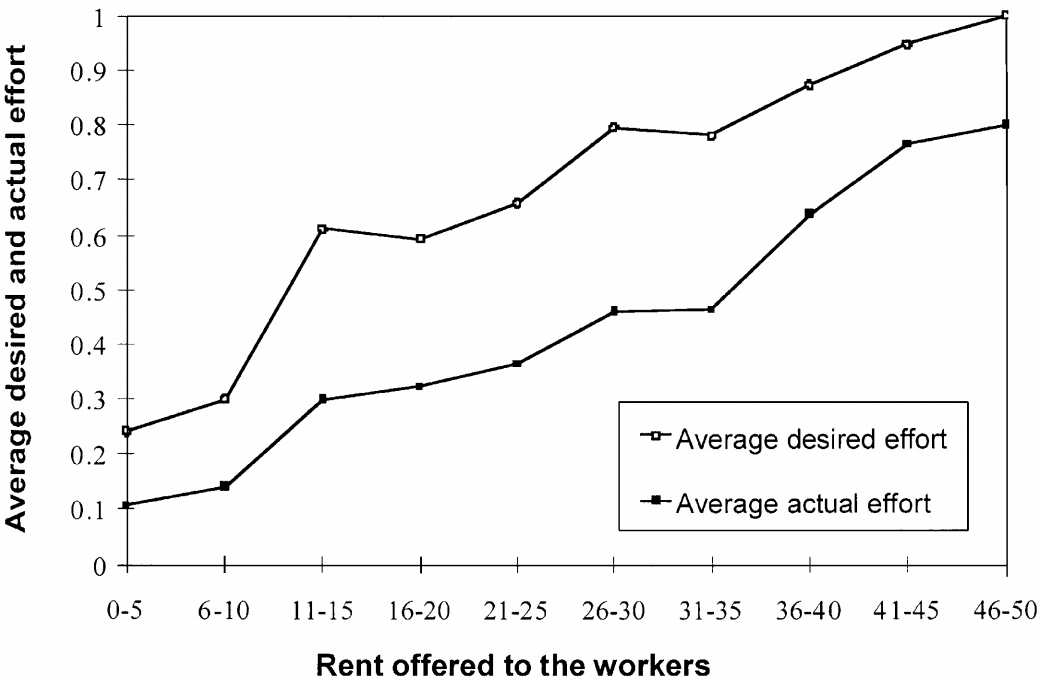
\includegraphics[scale=0.23]{effortwage.png}
			\caption{Fehr, E., \& Falk, A. (2002). Psychological foundations of incentives. European economic review, 46(4), 687-724.}
		\end{figure}
	\end{center}
\end{frame}


\begin{frame}
	\frametitle{Gift-Exchange game}
	
	\begin{itemize}
		\item The basic result of a positive relationship between effort level and wage has been replicated a number of times and appears robust.
	\end{itemize}
	However...
	\begin{itemize}	
		\item There has been pushback against the idea that laboratory results generalize to how people behave in the real world.
	\end{itemize}
	

	
\end{frame}

\section{The External Validity of Laboratory Experiments}

\AtBeginSection[]
{
	\begin{frame}{Table of Contents}
		\tableofcontents[currentsection]
	\end{frame}
}

\begin{frame}
	\frametitle{The External Validity of Laboratory Experiments}
	
	Do laboratory experiments tell us anything about economic behavior outside the lab? 
	
	\begin{itemize}
		\item \textbf{External Validity}: The ability of experiments to provide findings that allow for reliable inferences outside the laboratory
		\item A pernicious problem in the social sciences that does not exist to the same extent in the physical sciences
		\begin{itemize}
			\item E.g. It doesn't matter if you measure an object's acceleration due to gravity inside or outside the lab.
		\end{itemize}
	\end{itemize}
\end{frame}

\begin{frame}
	\frametitle{The External Validity of Laboratory Experiments}
	\textbf{Laboratory Experiments versus Field Studies}
	\begin{itemize}
		\item Laboratory experiments are often contrasted with field studies
		\item Field studies are touted as having more 'realistic' conditions, even if they're less tightly controlled
		\item Thus the findings from field studies are more externally valid than lab studies and are thus more relevant for policy decisions
	\end{itemize}

\end{frame}

\begin{frame}
	\frametitle{The External Validity of Laboratory Experiments}
	
	List, J. A. (2006) provides a good example of this.
	
	\begin{itemize}
		\item A gift-exchange game where buyers make price offers to sellers and sellers select the quality of the goods they provide.
		\begin{itemize}
			\item Standard prediction is that sellers provide the lowest quality possible and thus buyers offer the lowest price.
		\end{itemize}
		\item Instead of college students, the subjects were experienced sports-card traders.
		
	\end{itemize}
	
\end{frame}


\begin{frame}
	\frametitle{The External Validity of Laboratory Experiments}

	
	\begin{itemize}
		\item The results mirrored the typical findings of higher prices offered in exchange for goods of higher quality.
		\item In the second experiment, instead of an amorphous 'good', the subjects exchanged actual baseball cards of differing value and condition.
		\begin{itemize}
			\item The results were similar to the previous experiment.
		\end{itemize}
		\item For the third experiment List stepped outside the lab. Subjects were now in their natural environment: a sports-card show.
	\end{itemize}
\end{frame}

\begin{frame}
	\frametitle{The External Validity of Laboratory Experiments}
	
	\begin{itemize}

		\item In this field study there wasn't a relationship between price and quality.
		\begin{itemize}
			\item Only when there was concern for one's reputational standing was high offered price met with high quality offered
		\end{itemize} 
	\end{itemize}
\end{frame}

\begin{frame}
	\frametitle{The External Validity of Laboratory Experiments}
	
	How are we to adjudicate between findings from laboratory experiments and field studies? 
	
	Camerer, C (2015) distinguishes between the \textbf{scientific} and the \textbf{policy} view.
	\begin{itemize}
		\item In the policy view the external validity of the findings is of paramount importance thus field studies offer a surer way to study a proposed policy change.
		\item In the scientific view both laboratory experiments and field studies offer ways of enchancing our understanding of human behavior. Provided the evidence was properly gathered and is valid, there is no hierarchical relationship between the two.
	\end{itemize}
	
\end{frame}

\begin{frame}
	\frametitle{The External Validity of Laboratory Experiments}
	As Camerer puts it:
	
	\begin{aquote}{Colin Camerer, 2015}
		In this view, since the goal is to understand general principles, whether the 'lab generalizes to the field'...is distracting, difficult to know..., and is no more useful than asking whether 'the field generalizes to the lab'.
	\end{aquote}
	
\end{frame}

\begin{frame}
	\frametitle{The External Validity of Laboratory Experiments}

In the scientific view laboratory experiments and field studies are best viewed as completentary, each with their own strengths and weaknesses.

\begin{itemize}
	\item Laboratory experiments are easier to replicate.
	\item Field studies do a better job at collecting evidence for different subject pools
	\item Laboratory experiments are better positioned to explore a wider range of the parameter space	
\end{itemize}
	
	As Falk, A \& Heckman, J (2009) conclude, there is no a priori reason for prefering one over the other. They are both tools in the economist's toolbox. It ultimately boils down to a matter of the underlying research question and what tool is most appropriate to answer it.
	
\end{frame}

\section{Modelling Other-Regarding Preferences}

\AtBeginSection[]
{
	\begin{frame}{Table of Contents}
		\tableofcontents[currentsection]
	\end{frame}
}

\begin{frame}
	\frametitle{The Fehr-Schmidt Model of Inequity Aversion}
	
	Consider $n$ individuals, each with a respective monetary payoff $y_1,y_2,...,y_n$. For any $i$, the Fehr-Schmidt utility function, henceforth FS utility function, is defined as:
	
	\begin{equation}
	\begin{split}
	U_i\left(y_i,\vec{y}_{-i};\alpha_i,\beta_i\right) = y_i & -  \frac{\alpha_i}{n-1} \sum_{j\neq i} \max \left \{ y_j - y_i,0 \right \} \\
	& - \frac{\beta_i}{n-1} \sum_{j\neq i} \max \left \{ y_i - y_j,0 \right \}
	\end{split}
	\end{equation}

where $\alpha_i \geq \beta_i$ and $0 \leq \beta_i <1$.

\end{frame}

\begin{frame}
	\frametitle{The Fehr-Schmidt Model of Inequity Aversion}
\begin{columns}
	\begin{column}{0.5\textwidth}
		\begin{equation*}
			\frac{\alpha_i}{n-1} \sum_{j\neq i} \max \left \{ y_j - y_i,0 \right \} 
		\end{equation*}
		\begin{center}
			Disadvantageous Inequality
		\end{center}
		\begin{center}
		Envy
		\end{center}
	\end{column}
	\begin{column}{0.5\textwidth}  %%<--- here
		\begin{equation*}
\frac{\beta_i}{n-1} \sum_{j\neq i} \max \left \{ y_i - y_j,0 \right \}
\end{equation*}
\begin{center}
	Advantageous Inequality
\end{center}
\begin{center}
	Altruism
\end{center}
	\end{column}
\end{columns}
\end{frame}

\begin{frame}
	\frametitle{The Fehr-Schmidt Model of Inequity Aversion}
	\begin{center}
		\begin{figure}

			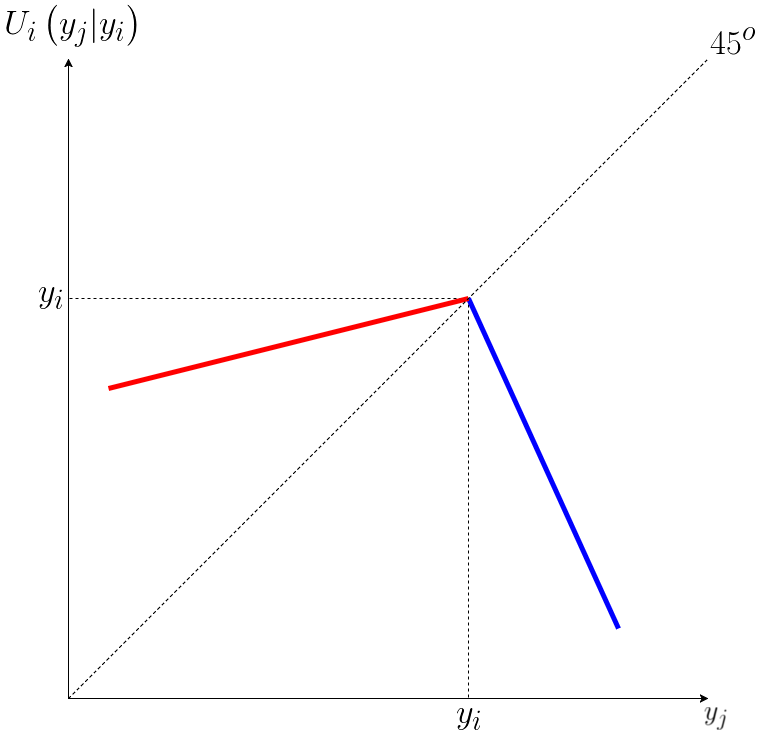
\includegraphics[scale=0.245]{fehrschmidt.png}

		\end{figure}
	\end{center}
	\begin{center}
	\begin{figure}
		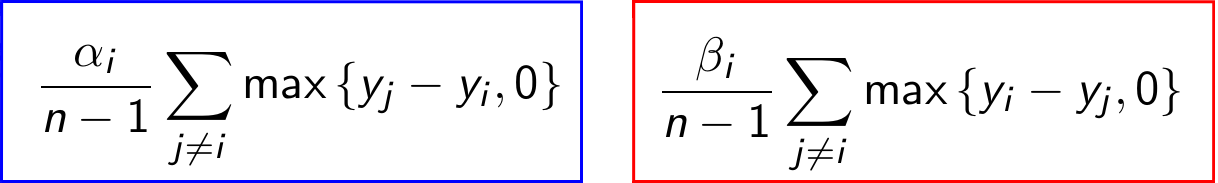
\includegraphics[scale=0.15]{eq.png}
	\end{figure}
\end{center}

	
\end{frame}
	
\begin{frame}
	\frametitle{The Fehr-Schmidt Model of Inequity Aversion}

	\textbf{Ultimatum Game}
	
	An Ultimatum Game is played between a Proposer and a Responder. THey are, respectively, Player 1 and Player 2. The share proposed is denoted by $s$
	
	\begin{lemma}
		The responder accepts all offers $s \geq 0.5$. There is a critical share, $s_c < 0.5$ such that the responder rejects all offers below it and accepts all offers $s \geq s_c$
	\end{lemma}
	
\end{frame}

\begin{frame}
		\frametitle{The Fehr-Schmidt Model of Inequity Aversion}
	\begin{proof}
	Taking into account the FS utility function for the case with only 2 players, we have the following for the responder:
	
	\begin{equation*}
	U_2 = s - \beta_2 \left[s - \left(1-s\right)\right]
	\end{equation*}
	
	which is positive because $\beta \in \left[0,1\right)$, hence the responder will accept.
	
	Now suppose $s<0.5$. In this case we have
	
	\begin{equation*}
	U_2 = s - \alpha_2 \left[\left(1-s\right) - s  \right] = s(1+2\alpha_2)-\alpha_2
	\end{equation*}
	
	For this to be positive we need $s$ such that 
	
	\begin{equation*}
	s \geq \frac{\alpha_2}{1+2\alpha_2}
	\end{equation*}
	
	Taking $\alpha \rightarrow \infty$ reveals that the critical threshold, $s_c$ is 0.5.
	
	\end{proof}
		
\end{frame}
	
\begin{frame}
	\frametitle{The Fehr-Schmidt Model of Inequity Aversion}

	\begin{prop}
	The equilibrium share offered by the proposer is given by:
	
		\begin{equation*}
			s^* =\left\{\begin{matrix}
			s_c & \text{if} & \beta_1 <0.5\\ 
			0.5 & \text{if}&\beta_1 >0.5\\ 
			s_ \in \left[s_c,0.5 \right] & \text{if}&\beta_1 =0.5
			\end{matrix}\right.
		\end{equation*}	
	\end{prop}

From the previous Lemma we know that the responder will accept any share $s_c \leq s \leq 0.5$.  Let us consider such a share.

\end{frame}	

\begin{frame}
		
	From the FS utility function we have, for the proposer 
	
	\begin{equation*}
			U_1 = \left(1-s\right) - \beta_1 \left[\left(1-s\right)-s\right]
	\end{equation*}
	
Taking the first derivative with respect to $s$ leaves us with $2\beta_1 -1$. Thus:

\begin{itemize}
	\item If $\beta_1 < 0.5$, we have $\frac{\partial U_1}{\partial s}<0$ so the proposer should offer the minimum possible that the responder will accept, i.e., $s_c$.
	\item 	If $\beta_1 = 0.5$ we have $\frac{\partial U_1}{\partial s}=0$ so any feasible share between $s_c$ and 0.5 may be offered and will be accepted.
	\item 	For values of $B_1$ higher than 0.5, $\frac{\partial U_1}{\partial s}>0$, so we have a corner solution where $s^* = 0.5$
\end{itemize} 	


\end{frame}


\section{Incomplete contracts under other-regarding preferences}

\AtBeginSection[]
{
	\begin{frame}{Table of Contents}
		\tableofcontents[currentsection]
	\end{frame}
}

\begin{frame}
	\frametitle{Incomplete contracts under other-regarding preferences}
	\centering
	
\includegraphics[scale=0.28]{UnderConstruct.png}
\end{frame}

\section{Conclusion}
\AtBeginSection[]
{
	\begin{frame}{Table of Contents}
		\tableofcontents[currentsection]
	\end{frame}
}

\begin{frame}
	\frametitle{Conclusion}
	\begin{itemize}
		\item As Aristotle put it once, "Man is by nature a social animal."
		\item Acknowledging the existence of other-regarding preferences allows economists to extend their studies by taking into account the social aspect of human behavior.
	\end{itemize}
\end{frame}
\section{References}
\begin{frame}
	\frametitle{References}
	\begin{itemize}
		\item Cameron, L. A. (1999). Raising the stakes in the ultimatum game: Experimental evidence from Indonesia. Economic Inquiry, 37(1), 47-59.
		Chicago	
		\item Andersen, S., Ertaç, S., Gneezy, U., Hoffman, M., \& List, J. A. (2011). Stakes matter in ultimatum games. The American Economic Review, 101(7), 3427-3439.
		\item Slonim, R., \& Roth, A. E. (1998). Learning in high stakes ultimatum games: An experiment in the Slovak Republic. Econometrica, 569-596.
		\end{itemize}

\end{frame}

\begin{frame}
	\frametitle{References}
	\begin{itemize}
		\item Camerer, C. F (2003). Behavioral Game Theory: Experiments in Strategic Interaction. Princeton University Press.
		\item Roth, A. E., Prasnikar, V., Okuno-Fujiwara, M., \& Zamir, S. (1991). Bargaining and market behavior in Jerusalem, Ljubljana, Pittsburgh, and Tokyo: An experimental study. The American Economic Review, 1068-1095.
		\item Akerlof, G. A. (1982). Labor contracts as partial gift exchange. The Quarterly Journal of Economics, 97(4), 543-569.
		\item List, J. A. (2006). The behavioralist meets the market: Measuring social preferences and reputation effects in actual transactions. Journal of political Economy, 114(1), 1-37.
	\end{itemize}
	
\end{frame}

\begin{frame}
	\frametitle{References}
	\begin{itemize}
		\item List, J. A. (2006). The behavioralist meets the market: Measuring social preferences and reputation effects in actual transactions. Journal of political Economy, 114(1), 1-37.
		\item Camerer, C. (2015). The promise and success of lab-field generalizability in experimental economics: A critical reply to Levitt and List. Handbook of Economic Methodology. Oxford University Press.
		\item Falk, A., \& Heckman, J. J. (2009). Lab experiments are a major source of knowledge in the social sciences. science, 326(5952), 535-538.
	\end{itemize}
	
\end{frame}

\end{document}